\documentclass[border=0mm,tikz]{standalone}


\usepackage{cmap}
% \usepackage[defaultsans]{droidsans}
% \renewcommand*\familydefault{\sfdefault} %% Only if the base font of the document is to be typewriter style
\usepackage[T2A]{fontenc}
\usepackage[utf8x]{inputenc}
\usepackage{amsmath,amssymb}
\usepackage{esdiff,esint}


\usepackage{pgfplots}
\usetikzlibrary{shapes, arrows}
\pgfplotsset{compat=1.10}
\usepgfplotslibrary{fillbetween}
\usetikzlibrary{patterns}
\usepackage[outline]{contour}

\def\centerarc[#1](#2)(#3:#4:#5);%
%Syntax: [draw options] (center) (initial angle:final angle:radius)
    {
    %\draw[#1] ($(#2)+({#5*cos(#3)},{#5*sin(#3)})$) arc (#3:#4:#5);
    \draw[#1]([shift=(#3:#5)]#2) arc (#3:#4:#5);
    }
\begin{document}

\begin{tikzpicture}%width=12cm,height=8cm]
\begin{axis}[axis lines=middle,
            xlabel={$g_1$},
            ylabel={$g_2$},
            scale=1.4,
            % width=12cm,
            height=8cm,
            % enlargelimits,
            unit vector ratio*=1 1 1,
            ytick=\empty,
            xtick=\empty,
            ymin=-2,
            ymax=2,
            xmin=-3,
            xmax=3,
            domain=-2:2, restrict y to domain=-2:2,
            % xtick={1,4},
            % xticklabels={a,b}
            ]

\xdef\From{0.5}
\xdef\To{3}

\path[name path=axisy] (axis cs:0,-2) -- (axis cs:0,2);
\path[name path=axisx] (axis cs:-\To,0) -- (axis cs:\To,0);
\path[name path=xmin] (axis cs:-\To,-2) -- (axis cs:\To,-2); 
\path[name path=xmax] (axis cs:-\To,2) -- (axis cs:\To,2);



\addplot[name path=A,blue,domain={\From:\To},samples=100] {1/x} node[pos=.8, above]{};

\addplot[name path=B,blue,domain={-\To:-\From},samples=100] {1/x} node[pos=.8, above]{};

\addplot[pattern=north east lines, pattern color=black!50]fill between[of=B and xmin, soft clip={domain=-\To:-\From}];

\addplot[pattern=north east lines, pattern color=black!50]fill between[of=A and xmax, soft clip={domain=\From:\To}];

\addplot[pattern=north east lines, pattern color=black!50]fill between[of=axisx and xmin, soft clip={domain=0:\To}];

\addplot[pattern=north east lines, pattern color=black!50]fill between[of=axisx and xmax, soft clip={domain=-\To:0}];

\draw [densely dashed, opacity=0.3] (axis cs:-2,-2) -- (axis cs:2,2);

\draw[dashed] (axis cs:-1,0) 
      -- (axis cs:-1,-1)
      -- (axis cs:0,-1);

\draw[dashed] (axis cs:1,0) 
      -- (axis cs:1,1)
      -- (axis cs:0,1);


% \contourlength{1cm}; 
\contourlength{1.2mm};

\coordinate (parallel)  at (axis cs:2,1.5);
\coordinate (ust)  at (axis cs:-1.5,1);
\coordinate (conc)  at (axis cs:-2.1,-1.5);
\coordinate (conf)  at (axis cs:1.5,-1);

\xdef\Scale{1}
% \contour{white}{}
\node[scale=1.1,align=center] at (ust)  {\contour{white}{Условие устойчивости:}\\\contour{white}{$0<g_1g_2<1$}\\\\\contour{white}{где}\\\\\contour{white}{$g_1=1-\frac{L}{R_1},\quad g_2=1-\frac{L}{R_2}$}};


\draw (parallel) node[scale=\Scale,align=center]  {\contour{white}{Плоские зеркала}\\\contour{white}{($R_1=R_2=\infty$)}}
node[inner sep=0pt, yshift=-1.5em, below] at (parallel)
    {
\includegraphics[width=7em]{parallel}}; 


\draw (conc) node[scale=\Scale,align=center]  {\contour{white}{Концентрические}\\\contour{white}{зеркала}\\\contour{white}{($R_1=R_2=L/2$)}} node[above,inner sep=0pt,yshift=1.7em] 
    {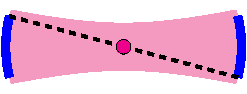
\includegraphics[width=7em]{conc}};



\draw (conf) node[inner sep=0pt,above]
    {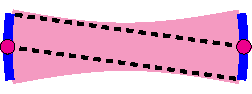
\includegraphics[width=7em]{conf}} node [below, align=center,scale=\Scale] {\contour{white}{Конфокальные}\\\contour{white}{зеркала}\\\contour{white}{($R_1=R_2=L$)}};
% \node[coordinate,pin=30:{$A$}] at (axis cs:3.8,3){};

\coordinate (A) at (axis cs:0.7,-0.75);
\coordinate (0) at (axis cs:0,0);
% \draw (A) -- (0);
\path[draw] (A) edge [out=180, in=-80,->, thick, >=latex] (0);

\draw[fill=magenta] (axis cs:0,0) circle (2pt);

\draw[fill=magenta] (axis cs:1,1) circle (2pt) node[left, yshift=-1em, scale=0.8]{\contour{white}{$(1,1)$}};

\draw[fill=magenta] (axis cs:-1,-1) circle (2pt) node[right, yshift=1em, scale=0.8]{\contour{white}{$(-1,-1)$}};

\end{axis}
\end{tikzpicture}

% \begin{tikzpicture}
% \begin{axis}[axis lines=middle,
%             xlabel=$x$,
%             ylabel=$y$,
%             enlargelimits,
%             ytick=\empty,
%             xtick={-2.19,2.19},
%             xticklabels={$x_1$,$x_2$}]
% \addplot[name path=F,blue,domain={-4:4}] {-(1/6)*x^2+2} node[pos=1, below]{$f$};

% \addplot[name path=G,green,domain={-4:4}] {0.25*x^2}node[pos=1, above]{$g$};

% \addplot[pattern=north west lines, pattern color=brown!50]fill between[of=F and G, soft clip={domain=-2.19:2.19}]
% ;
% \node[coordinate,pin=60:{$A$}] at (axis cs:1.1,1.6){};

% \end{axis}
% \end{tikzpicture}
\end{document}